% Data Flow Diagram
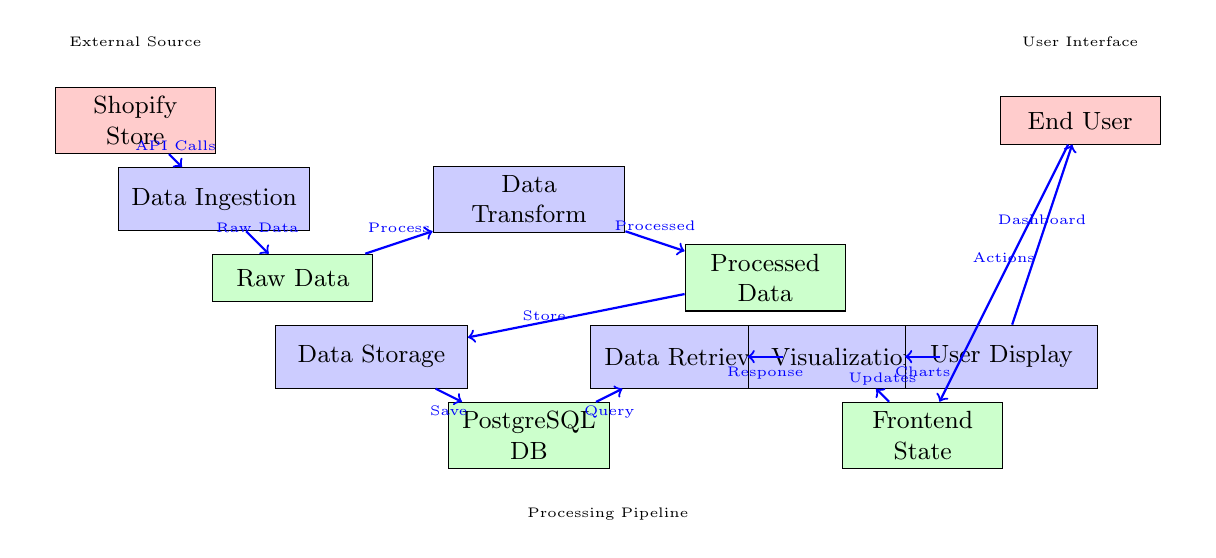
\begin{tikzpicture}[
    node distance=2.5cm,
    process/.style={rectangle, draw, fill=blue!20, text width=2.2cm, text centered, minimum height=0.8cm, font=\small},
    data/.style={rectangle, draw, fill=green!20, text width=1.8cm, text centered, minimum height=0.6cm, font=\small},
    external/.style={rectangle, draw, fill=red!20, text width=1.8cm, text centered, minimum height=0.6cm, font=\small},
    arrow/.style={->, thick, blue},
    label/.style={text width=2.5cm, text centered, font=\tiny}
]

% External entities
\node[external] (shopify) at (0, 10) {Shopify Store};
\node[external] (user) at (12, 10) {End User};

% Data stores
\node[data] (rawdata) at (2, 8) {Raw Data};
\node[data] (processed) at (8, 8) {Processed Data};
\node[data] (database) at (5, 6) {PostgreSQL DB};
\node[data] (frontend) at (10, 6) {Frontend State};

% Processes
\node[process] (ingestion) at (1, 9) {Data Ingestion};
\node[process] (transformation) at (5, 9) {Data Transform};
\node[process] (storage) at (3, 7) {Data Storage};
\node[process] (retrieval) at (7, 7) {Data Retrieval};
\node[process] (visualization) at (9, 7) {Visualization};
\node[process] (display) at (11, 7) {User Display};

% Data flows
\draw[arrow] (shopify) -- node[above, font=\tiny] {API Calls} (ingestion);
\draw[arrow] (ingestion) -- node[above, font=\tiny] {Raw Data} (rawdata);
\draw[arrow] (rawdata) -- node[above, font=\tiny] {Process} (transformation);
\draw[arrow] (transformation) -- node[above, font=\tiny] {Processed} (processed);
\draw[arrow] (processed) -- node[left, font=\tiny] {Store} (storage);
\draw[arrow] (storage) -- node[below, font=\tiny] {Save} (database);
\draw[arrow] (database) -- node[below, font=\tiny] {Query} (retrieval);
\draw[arrow] (retrieval) -- node[below, font=\tiny] {Response} (visualization);
\draw[arrow] (visualization) -- node[below, font=\tiny] {Charts} (display);
\draw[arrow] (display) -- node[above, font=\tiny] {Dashboard} (user);

% Feedback loop
\draw[arrow] (user) -- node[above, font=\tiny] {Actions} (frontend);
\draw[arrow] (frontend) -- node[above, font=\tiny] {Updates} (visualization);

% Labels
\node[label] at (0, 11) {External Source};
\node[label] at (12, 11) {User Interface};
\node[label] at (6, 5) {Processing Pipeline};

\end{tikzpicture}
